\documentclass[twoside,11pt,openright]{report}

\usepackage[utf8]{inputenc}
\usepackage[american]{babel}
\usepackage{a4}
\usepackage{natbib}
\usepackage{latexsym}
\usepackage{mathtools}
\usepackage{amssymb}
\usepackage{amsmath}
\usepackage{amsthm}
\usepackage{epsfig}
\usepackage[T1]{fontenc}
\usepackage{lmodern}
\usepackage[labeled]{multibib}
\usepackage{color}
\usepackage{datetime}
\usepackage{epstopdf} 
\usepackage{cleveref}
\usepackage{geometry}
\usepackage{tikz}
\usepackage[]{algorithm2e}
\usepackage{graphicx}

\renewcommand*\ttdefault{txtt}

\newcommand{\todo}[1]{{\color[rgb]{.5,0,0}\textbf{$\blacktriangleright$#1$\blacktriangleleft$}}}
\newcommand{\DIST}{\operatorname{DIST}}

\newcommand{\substr}[3]{#1\langle #2, #3 \rangle}
\newcommand{\str}[3]{#1[#2, #3]}
\newcommand*{\circled}[1]{\tikz[baseline=(char.base)]{
                          \node[shape=circle,draw,inner sep=2pt] (char) {#1};}}

\newcommand{\ceil}[1] {\lceil #1 \rceil}
\newcommand{\SLP}[1] {\mathcal{#1}}

\newcommand{\refbook}[2]{\cite[#1]{DBLP:journals/corr/abs-0707-3619}, #2}
\newcommand{\reftiskin}[2]{\cite[#1]{Tiskin:2010:FDM:1873601.1873704}, #2}

\newcites{A,B}{Primary Bibliography,Secondary Bibliography}

\newtheorem{mydef}{Definition}
\newtheorem{problem}{Problem}
\newtheorem{claim}{Claim}
\newtheorem{lemma}{Lemma}
\newtheorem{theorem}{Theorem}

% see http://imf.au.dk/system/latex/bog/

\crefname{algocfline}{algorithm}{algorithms}

\begin{document}

\RestyleAlgo{boxruled}
\LinesNumbered

%%%%%%%%%%%%%%%%%%%%%%%%%%%%%%%%%%%%%%%%%%%%%%%%%%%%%%%%%%%%%%%%%%%%%%%

\pagestyle{empty} 
\pagenumbering{roman} 
\vspace*{\fill}\noindent{\rule{\linewidth}{1mm}\\[4ex]
{\Huge\sf Computation of Edit Distance in Compressed Strings}\\[2ex]
{\huge\sf Kasper Nielsen, 20091182}\\[2ex]
\noindent\rule{\linewidth}{1mm}\\[4ex]
\noindent{\Large\sf Master's Thesis, Computer Science\\[1ex] 
\monthname\ \the\year  \\[1ex] Advisor: Christian Nørgaard Storm Pedersen\\[15ex]}\\[\fill]}

\epsfig{file=logo.eps}\clearpage

%%%%%%%%%%%%%%%%%%%%%%%%%%%%%%%%%%%%%%%%%%%%%%%%%%%%%%%%%%%%%%%%%%%%%%%

\pagestyle{plain}
% \chapter*{Abstract}
% \addcontentsline{toc}{chapter}{Abstract}

% \todo{in English\dots}

% \chapter*{Resum\'e}
% \addcontentsline{toc}{chapter}{Resum\'e}

% \todo{in Danish\dots}

% \chapter*{Acknowledgements}
% \addcontentsline{toc}{chapter}{Acknowledgments}

% \todo{\dots}

% \vspace{2ex}
% \begin{flushright}
%   \emph{Kasper Nielsen,}\\
%   \emph{Aarhus, \today.}
% \end{flushright}

\tableofcontents
\pagenumbering{arabic}
\setcounter{secnumdepth}{2}

%%%%%%%%%%%%%%%%%%%%%%%%%%%%%%%%%%%%%%%%%%%%%%%%%%%%%%%%%%%%%%%%%%%%%%%

\chapter{Introduction}
\label{ch:intro}

This report will focus on the computation of edit distance in compressed strings. The edit distance is a measure of how similar or dissimilar two string are. More precisely,
\begin{problem}
  \label{problem:edit-distance}
  The edit distance between two strings $\str{A}{0}{m}$ and $\str{B}{0}{n}$ counts the minimum number of operations needed to transform $A$ into $B$. The set of the available operations are to: insert a character, delete a character or to substitute a character by another. Each of the operations is associated with a cost. Throughout the thesis the Levenshtein distance will be used, where the cost of a substitution is 0 on a match and 1 otherwise. Insert and delete operations have cost 1.
\end{problem}

The scores could be generalized to other constants, but also to arbitrary functions. Different choices may result in more complicated algorithms with worse asymptotic running time and space consumption, even if the cost function is assumed to be computable in constant time. However, this thesis will only focus on the edit distance problem as defined in \cref{problem:edit-distance}, and how fast this can be computed in compressed strings.

\section{Work contribution}
The main focus of this thesis is based on the algorithm described in \cite{Gawrychowski:2012:FAC:2422024.2422048} which builds on top of the approach described in \cite{DBLP:journals/corr/abs-1004-1194} and \cite{DBLP:journals/corr/abs-0707-3619}. To this date, this is the asymptotically best known algorithm in the RAM for computation of edit distance in strings encoded by straight-line programs (SLPs). Given two input strings $\str{A}{0}{k}$ and $\str{B}{0}{l}$ the algorithm runs in time $O(n N \sqrt{\log{\frac{N}{n}}})$, where $N = k + l$ and $n$ is the sum of the number of productions in the SLP representation of the input strings (see \cref{ch:compressing-strings}). It is a open problem if the running time can be reduced to $O(nN)$, which is a bit further discussed in \cref{sec:conclusion:further-work}.

This thesis has a two-fold objective. First and foremost to implement the algorithm and benchmark it to see how the technique performs in practice. The second objective is to give a coherent description of the algorithm and prove that it works. The proofs follow the ones presented in \cite{DBLP:journals/corr/abs-0707-3619} \todo{give range on proofs?}, but the proofs supplied in this report are in many cases more thorough and detailed.

The following list of algorithms has been implemented in order to test the algorithm in practice:
\todo{Consider if this should be moved until a point where terminology is defined.}
\begin{itemize}
  \item The SLP construction algorithm of \cite{Rytter2003211}. The algorithm is further described in \cref{ch:compressing-strings}.
  \item Algorithm as described in \cite{DBLP:journals/corr/abs-1004-1194} for dividing the input strings into blocks of size $O(x)$ for some $x$, corresponding to productions in the SLP. The algorithm is described in \cref{sec:algorithm:select-productions}.
  \item Algorithm from \cite{DBLP:journals/corr/abs-1004-1194} for building DIST tables based on the input string partitions. Described in \cref{sec:algorithm:building-DISTs-overview}.
    \begin{itemize}
      \item This algorithm requires the ability to min-multiply two simple unit-Monge matrices given by \cite{Tiskin:2010:FDM:1873601.1873704}. This algorithm is described in \cref{sec:algorithm:min-mult-two-unit-monge}.
    \end{itemize}
  \item Algorithm for filling out the dynamic programming table using the DISTs, see \cref{sec:algorithm:filling-grid-overview}.
    \begin{itemize}
      \item An algorithm for max-multiplying a DIST with an arbitrary vector from \cite{Gawrychowski:2012:FAC:2422024.2422048} running in linear time. This algorithm is described in \cref{sec:algorithm:max-mult-H-table-with-vector}.
      \item The max-multiply algorithm further relies on an interval union find data-structure from \cite{Itai06lineartime}. Described in \cref{sec:algorithm:interval-union-find}.
    \end{itemize}
\end{itemize}
The algorithm for constructing the SLP encoding of the input strings requires a suffix tree. In order to have a succinct and efficient suffix tree, it has been chosen to use a suffix tree implementation in the Succinct Data Structure Library (SDSL) \cite{SDSL} based on \cite{OHL:FIS:GOG:2010}.

\section{Implementation and test setup}
All measurements presented in this report were performed on a computer with an Intel i5-4258U CPU with the following technical specifications:
\begin{itemize}
  \item 2 cores operating at 2.4GHz, with turbo boost up to 2.9GHz.
  \item 256KB L2 cache, 3MB L3 cache.
\end{itemize}
The main memory size of the machine is 16 Gb. The computer was running Mac OS X and Intel Performance Counter Monitor (IPCM) was used to measure cache misses and instructions executed. All implementations have been written in \texttt{C++11} and compiled on  Mac OS X using the clang 3.3 compiler. When measurements were performed, the code was compiled using the \texttt{-O3 -funroll-loops -flto -fasm-blocks -march=core-avx2 -DNDEBUG} optimization flags.

Before doing the actual measurements, a small warm-up round was performed, ensuring that the code was in the CPU cache etc. This helped to greatly reduce the variance of the running time measurements yielding more consistent results.

All running times was measured as wall-time, and all tests was repeated 5 times where the measurement with the median running times is the one used for data-analysis in this report. The reason for choosing the median measurement, is that an unexpected amount of machine activity in one of the trials should not penalize the result, but at the same time, some tasks done by the operating system may be needed for the algorithm to function, which is why the minimum time was not selected. However, the variation between the trails was found to be very small \todo{check this, and report RSD?}.

\subsubsection{Correctness}
In order to verify the correctness of the implementation, the result has been checked up against the simple algorithm described in \cref{sec:intro:simple}. Also, unit tests have been made to individually test parts of the algorithm, and during debugging and testing a lot of consistency checks are performed on every run. There are no known bugs in the implementation. 

\section{Simple algorithm}
\label{sec:intro:simple}
A standard dynamic programming algorithm for solving the edit distance problem, here denoted the simple algorithm\todo{Credit someone?}. It is given two string $\str{A}{1}{m}$ and $\str{B}{1}{n}$ for which the edit distance should be computed, and fills out a matrix of size $m \times n$ where a given entry $(i, j)$ corresponds to the edit distance between $\str{A}{1}{i}$ and $\str{B}{1}{j}$. The rules for filling out a table entry follows directly from the definition of edit distance when extending a string, and are as follows:
\[
  T[i, j] = \max \left\{ \begin{array}{lll}
              T[i - 1, j - 1] + \delta(A[i], A[j]) & \text{if } i, j \geq 1 & \text{Match} \\
              T[i - 1, j] + 1       & \text{if } i \geq 1, j \geq 0       & \text{Insert} \\
              T[i, j - 1] + 1       & \text{if } i \geq 0, j \geq 1       & \text{Delete}
            \end{array} \right.
\]
where
\[
  \delta(a, b) = \begin{cases}
                   0 & \text{if } a = b \\
                   1 & \text{o/w.}
                 \end{cases}
    \quad \text{ for } \quad a, b \in \Sigma.
\]
The base case where a string is aligned to the empty string is trivially the length of the non-empty string. Therefore the edit distance between two string can be computed using both $O(nm)$ time and space. Notice that an easy optimization where only the last row used is stored in memory reduces the space consumption to $O(\min\{n, m\})$.

\subsection{Backtracking}
If the actual alignment of the strings is desirable, it can be found by a standard back-tracking approach on the computed matrix.

This however implies that the simple space optimization from before does not work, as all entries in the computed table potentially is needed for the backtracking. However, a divide-and-conquer algorithm was given by Hirshberg\todo{Cite} that reduces the space consumption of $O(\min\{n, m\})$ without asymptotically increasing the running time.\todo{Describe the approach?}

The same approach can be used to find the alignment for the main algorithm in this report. However, a more practical approach may be to use the simple algorithm with pruning when the known optimal score is known, and then use backtracking directly on the grid. From now on, only the actual edit distance is considered to be of interest.

\subsection{Optimizations}
Ideas:
\begin{itemize}
  \item Compute matrix only around its diagonal, and then extend if needed. Extend by powers of $2$, which will result in at most a factor of $2$ extra running time.
  \item Using SIMD instructions.
  \item Parallelization (CPU / GPU).
\end{itemize}

In order to bound the scope of this thesis, it has been chosen not to focus on parallelization of the algorithms, even through both the simple and the main algorithm investigated in this thesis of \cite{Gawrychowski:2012:FAC:2422024.2422048} should be easily parallelizable. For more details see \ref{sec:conclusion:further-work}.

\section{Compression based algorithms}
There exists other approaches for speeding up the computation of the edit distance between two strings. This section presents a short overview of some of the approaches that relates to the approach investigated in this thesis.

One approach for speeding up the computation of edit distance, is to compress the input strings, and then in some way do the edit distance computation using the compressed strings, which for many cases will be shorter than the original input.

\subsection{The 4 Russian Algorithm}
This approach was not originally presented as a compression based algorithm, but using that each entry in the dynamic programming matrix is changing at most 1 from an adjacent entry, and that the alphabet is finite, it is possible to encode blocks of the dynamic programming table efficiently and pre-compute all of them. That is, for all different sub-strings and possible inputs to compute the relative outputs when applying the block. Due to that values can change by no more than $1$ between two entries, the representation can be succinctly represented and efficiently looked up. The pre-computed tables are then used to fill out the original dynamic programming matrix block-by-block.
\todo{Describe details and analyze time complexity?.}

\subsection{Run-Length Encoding}
\begin{itemize}
  \item \todo{Describe RLE}
  \item Not the focus / implemented in this thesis, but the result is included for completeness. Refer old thesis for experimental results of this approach?
  \item \todo{cite} gave an algorithm running in time $O(nm)$ where $n$ and $m$ denotes the size of the compressed sequences. This is the first result where the running time is only depending on the length of the compressed strings. However, for string not containing long runs of the same symbol, RLE will generate strings longer than the original input!
\end{itemize}

\subsection{Compression based on straight-line programs}
This section gives a very brief overview of the algorithm given by \cite{Gawrychowski:2012:FAC:2422024.2422048}, which is the main focus of this thesis. A more detailed description of each of the steps of the algorithm will be given later in this report. 

Another way of compressing a string, is to compress it to what is known as a straight-line program (SLP). A more formal definition of a SLP will be given in \cref{ch:compressing-strings}, for now it is sufficient to note that a SLP is a restricted context-free grammar.

The algorithm can be seen as a generalization of the 4-Russian approach, where the blocking of the dynamic programming table is based on the productions of the SLPs, so that reused productions result in reusable blocks when filling out the grid. The algorithm can be summarized in the following steps:
\begin{itemize}
  \item Construct SLP representations $\SLP{A}$, $\SLP{B}$ of the two input strings $\str{A}{0}{m}$ and $\str{B}{0}{n}$. The better the compression scheme is able to compress the SLP representations the faster the algorithm will be. A natural trade-off arises in this step, namely the running time of the compression scheme versus the quality of the resulting compression. This step will be discussed in \cref{ch:compressing-strings}.
  \item Productions from the SLPs generating strings of length $O(x)$ for some fixed $x$ are selected in such a way that they cover the entire string without duplication. This can be done in $O(N)$ time by traversing the productions of the SLP bottom-up as described in \cref{sec:algorithm:select-productions}.
  \item Blocks from the dynamic programming table are precomputed for all the selected productions (these precomputed tables are called DIST tables). By naively representing the DIST tables they each take up $O(x^2)$ space, but using a succinct representation given in \cite{DBLP:journals/corr/abs-0707-3619}, it is possibly to reduce the space consumption to $O(x)$ and also improve the time it takes to use a $\DIST$. This step is described in \cref{sec:algorithm:building-DISTs-overview}.
  \item The dynamical programming table is filled up by using the partition and the precomputed $\DIST$ tables. This step takes time $O\left(\left(\frac{N}{x}\right)^2 \cdot AP(x)\right)$ where $AP(x)$ is the time to apply a DIST table. Using the succinct representation, \cite{Gawrychowski:2012:FAC:2422024.2422048} shows how to make $AP(x) = O(x)$, leading to a total running time of $O(\frac{N^2}{x})$. This step is described in \cref{sec:algorithm:filling-grid-overview}.
\end{itemize}

\chapter{Compressing input strings}
\label{ch:compressing-strings}
There exist are large number of compression schemes for compressing strings, spanning both lossy and lossless schemes. Since it is desired that the edit distance algorithm always gives the correct result, only lossless compression schemes are considered.

The algorithm examined in this thesis is working over straight-line programs (SLPs), whereby only compression to these formats are considered.
\begin{mydef}
  A straight-line program (SLP) is a restricted context-free grammar $G = (V, T, R, S)$, where
  \begin{itemize}
    \item $V = \{ S_1, \dots, S_n\}$ is a ordered set of non-terminals
    \item $T = \{ S_{n + 1}, \dots, S_{n + m} \}$ is a ordered set of terminals
    \item $R$ is a set of production rules mapping $V$ to $(V \cup T)^2$, with the condition that if $(S_i \to S_jS_k) \in R$, then $j,k \geq i$. This ensures that a SLP generates exactly one string.
    \item The start production $S = S_1$.
  \end{itemize}
  The size of a SLP is defined to be $|V \cup T|$, which is only a constant from the actual space consumption of a simple pointer-based SLP implementation.
\end{mydef}
From this definition it is not possible for a SLP to generate the empty string, however this poses no problem in practice as that case can be handled separately.
\begin{problem}
  \label{compression:problem:minimum-slp}
  Given an input string $\str{A}{0}{m}$ find a SLP $\SLP{A}$ of minimum size generating $A$.
\end{problem}
It is known \cite[p. 212]{Rytter2003211} that this problem is NP-complete, hence a general, exact and efficient algorithm should not be expected to be easily obtainable. However, a number of articles (ex. \cite{Rytter2003211} and \cite{Sakamoto2005416}) has studied how to approximate a minimum size SLP for the input string. The approach implemented in this article is a $O(\log{n})$-approximation given in \cite{Rytter2003211}, which is based on the Lempel-Ziv factorization (LZ-factorization), which is a version of the popular LZ77 compression scheme \todo{cite?}. The algorithm is described in \cref{sec:compression:alg}.

A small theoretical improvement was given in \cite{Rytter2003211}, reducing the approximation factor to $O(\log{\frac{n}{g^*}})$ where $g^*$ denotes the size of the minimal SLP compression. As suggested by \cite{Rytter2003211} the improvement is mostly cosmetic, and from the description of the approach, I \todo{be sure} find it very likely that the approach will significantly increase the constant in front of the big-$O$ notation. Therefore, I have not chosen to implemented this theoretical improvement.

For computing the LZ-factorization a suffix tree is used. Suffix tress often comes with a large constant space overhead, making them undesirable in practice in some cases. \cite{Sakamoto2005416} gave another algorithm for solving \cref{compression:problem:minimum-slp} which also actives the $O(\log{\frac{n}{g^*}})$ approximation factor, but does it based on the RE-PAIR encoding scheme, which can be made to work without using a suffix tree. The reason for not implementing this approach, is that I find the LZ-factorization approach more intuitive, and that by experiments \todo{ref} it was found that the suffix-tree was not the limiting space consumer.

In other areas of lossless compression, ex. bzip2 compression, the input string is encoded using a Burrows-Wheeler transform (BWT) \cite{BurrowsWheeler}. The intuition that the BWT works, is that it permutes the string in such a way that highly repetitive parts of the string are group together, making them easier to compress. However building the SLP over the BWT of the input string will not work because the BTW permutes the string, such that productions of the SLP does not corresponds to a continuous area in the input string. I have not been able to find any articles able to take advantage of the BWT for SLP based compression.

In lossless compression there exists Entropy-based encoding schemes. Such schemes uses the frequencies of the appearing alphabet symbols in the string to compress them to use as few bits as possible. This type of compression is not of significant interest in this context, since we are only interest in minimizing the number of productions in the resulting SLP. However, one thing to notice is that an absolute lower bound when losslessly encoding a string exists, which is given by its entropy.
\todo{Talk about entropy, and relate to SLP?}

\paragraph{Notes about size}
Given input strings over the finite alphabet $\Sigma$, all strings over this alphabet can trivially be encoded using $\ceil{\log_2 |\Sigma|}$ bits per symbol. However, for a direct representation of the SLP using pointers a left and a right pointer has to be stored together with the symbol, which on a new machine uses up $64$ bits each. Moreover, the algorithms working on the SLPs are likely to require more information annotated to each node in the tree. This results in a huge constant blow up on the space required to store the input string, especially for strings not compressing very well.

It could be both of practical and theoretical interest to try to find a succinct representation of a SLP, in order to make the space consumption smaller, making the SLP approach practical for long strings that only compresses by around a constant factor.

\section{Algorithm}
\label{sec:compression:alg}
The idea behind the algorithm is to iteratively build the SLP for the string, by adding a repeating factor in the string once at a time. The repeating factor is added by reusing the productions in the SLP generating the factor. After each iteration, the (unique) parse tree of the SLP is considered as a AVL-tree and is balanced using appropriate AVL-tree rotations. An overview of the algorithm is given in \cref{alg:compression:approx}.

The $Concat$ process referenced in the code, is function almost the same way as concatenating two AVL trees \todo{see something}. However, nodes (productions) in the SLP parse tree may be shared, hence when adding nodes and making rotations, special care needs to be taken in order to ensure the balance of the tree, and that the derived string is correct. However, this is easy to fix, by simple introducing a constant number of new productions for every insertion and rotation. Amortized, the number of rotations that happens on every concatenation is constant, hence only a constant number of extra productions are added every time $Concat$ is called.

The factors iteratively added to the SLP are the LZ-factors of the input string $\str{A}{0}{m}$. \todo{Describe what LZ factors are.}

It is required to be able to efficiently find the nodes in the current SLP which generates a LZ factor. In order to do this, the LZ factors of the string are specified by their first occurrence in the input string by indices. Using these indices it is easy to find the corresponding productions in the SLP by annotating the derived length for each of the productions, and then make a top-down decent of the tree checking if the indices overlaps the current node.

\begin{algorithm}[H]
  \label{alg:compression:approx}
  Let $\SLP{A}$ be an empty SLP\;
  Construct LZ-Factorization $f_1,\dots,f_k$ of the input string $\str{A}{0}{m}$\;
  \For{$i = 1, \dots, k$}{
    Find productions $S_1,\dots,S_{k_i}$ in the current SLP $\SLP{A}$ generating $f_i$\;
    Set $\SLP{S} = Concat(S_1,\dots,S_{k_i})$\;
    $\SLP{A} = Concat(\SLP{A}, \SLP{S})$\;
  }
  \Return $\SLP{A}$
  \caption{Algorithm for generating $\log{n}$ approximation of minimal SLP of input string $\str{A}{0}{m}$.}
\end{algorithm}

The only step in the SLP construction that is not fully specified in \todo{cite}, is how to compute the LZ-factorization of a string efficiently. They only state that it can be done efficiently using a suffix tree. Although the algorithm is very simple, it is included in this report for completeness.

First the suffix tree for the input string is generated. Then every node $v$ in the tree is annotated with the first index in the string where the substring spelled out from the root to $v$ occurs. This is done by traversing the tree bottom up where all leafs are marked by their suffix numbers, and for any parent the minimum of their children is chosen.

Having the described suffix tree, the LZ-factorization can be found by searching in the suffix tree guided by a start position in the string and checking if the corresponding path was already seen in the string. Pseudo code for the algorithm is given in \cref{alg:compression:lz-factorization}.\todo{Implement this in code instead of slowscanning!}

\begin{algorithm}[H]
  \label{alg:compression:lz-factorization}
  $LZFactors = \emptyset$\;
  $i = 0$\;
  \While{$i < m$}{
    $start = i, edgeLength = 0$\;
    $currentNode = Root$\;
    \While{$FirstSeen[Root \to currentNode] < start$ and $i < m$}{
      $edgeFollowed, newNode = \operatorname{Follow}(curPos, A[i])$\;
      $edgeLength =$ length of $edgeFollowed$\;
      $currentNode = newNode$\;
      $i = i + edgeLength$\;
    }
    \eIf{$edgeLength == 0$}{
      $LZFactors = LZFactors \cup \{ A[start] \}$\;
      $i = i + 1$\;
    }{
      $LZFactors = LZFactors \cup \{ \substr{A}{start}{i - edgeLength} \}$\;
    }
  }
  \Return $LZFactors$
  \caption{Algorithm for generating the LZ-factorization of a given input string $A$. The algorithm assumes a $FirstSeen$ array that for a given node gives the first time its associated string occurs in the string.}
\end{algorithm}

\section{Benchmarks}
\label{sec:compression:benchmarks}

\chapter{SLP based edit distance algorithm}
\label{ch:algorithm}

This chapter will describe and benchmark the algorithm for computing the edit distance of two input SLPs $\SLP{A}$ and $\SLP{B}$.

\section{Preliminaries}
\label{sec:algorithm:preliminaries}
In order to describe the algorithm and argue its correctness, some notation will be introduced.

It has been chosen that all matrices used in this report are $0$-indexed. That is, an entry in a matrix $A$ of size $m \times n$ is indexed by $A(i, j)$ where $i \in \{0, \dots, m - 1\}, j \in \{0, \dots, n - 1\}$. Note that this is a different choice than the referenced literature describing the algorithm (most notably \cite{Tiskin:2010:FDM:1873601.1873704} and \cite{DBLP:journals/corr/abs-0707-3619}), who for convenience use odd half-integers to index some of the matrices. This approach was not chosen in order to make the calculations in this report closer to the actual \texttt{C++} implementation.

Almost all matrices considered in this report will be square matrices, ie. of size $n \times n$ for some $n \in \mathbb{N}$. Therefore all following definitions will only be given for square matrices, but most of them could easily be generalized to matrices of arbitrary dimension.

\begin{mydef}
  A permutation matrix of size $n$ is a matrix over $\{0,1\}^{n \times n}$ where each row and each column contains exactly one $1$. That is, it can be seen as the identity matrix of size $n \times n$ where the rows (or columns) are permuted.
  It is assumed that the index of the column (row) containing the $1$ can be found in constant time from a given row (column).
\end{mydef}
The latter constraint on the query time of the $1$ entry is required to achieve the running time of some of the algorithms (ex \todo{ref}). The way permutation matrices are represented in the implementation, is that the row and column permutation is specified using $2n = O(n)$ machine words. This directly gives the constant time query to the $1$ entry of a given row/column.

The algorithm stores a lot of permutation matrices in memory. It is therefore interesting to try to minimize the space consumption of these matrices. However, it turns out that the space consumption of $O(n)$ machine words is asymptotically optimal: A permutation matrix of size $n$ can express $n!$ different permutation matrices (since there are $n!$ different permutations of the rows of the identity matrix), hence at least $\Omega(\log{n!})$ bits are needed to represent a permutation matrix. By Stirling's approximation it is known that
\[
  \ln{n!} = n \ln{n} - n + O(\ln{n}),
\]
hence $\Omega(\log{n!}) = \Omega(n \log{n})$ bits are required to represent the permutation matrix, which is also what is used in the row/column-permutation representation.
%
\begin{mydef}
  The distribution matrix $A^{\Sigma}$ of a $n \times n$ matrix $A$ is a $(n + 1) \times (n + 1)$ matrix defined as
  \[
    A^{\Sigma}(i, j) = \sum_{\substack{\hat{i} \in \{i, \dots, n - 1\} \\ \hat{j} \in \{0, \dots, j - 1\}}} {A(\hat{i}, \hat{j})},
  \]
  or informally the sum of all entries in the sub-matrix to the left and below of a given entry $(i, j)$.
\end{mydef}
%
\begin{mydef}
  The density matrix $A^{\Box}$ of a $(n + 1) \times (n + 1)$ matrix is a $n \times n$ matrix defined as
  \[
    A^{\Box}(i, j) = A(i, j + 1) - A(i, j) - A(i + 1, j + 1) + A(i + 1, j)
  \]
  for all $i, j \in \{ 0, \dots, n - 1 \}$. \todo{Graphical representation?}
\end{mydef}%
Notice that for a any matrix $A$ of size $n \times n$ it is the case that \\
\scalebox{0.9}{\parbox{.5\linewidth}{%
\begin{align*}
  (A^{\Sigma})^\Box(i, j) &= A^{\Sigma}(i, j + 1) - A^{\Sigma}(i, j) - A^{\Sigma}(i + 1, j + 1) + A^{\Sigma}(i + 1, j) \\
    &= \sum_{\substack{\hat{i} \in \{i, \dots, n - 1\} \\ \hat{j} \in \{0, \dots, j\}}} {A(\hat{i}, \hat{j})}
     - \sum_{\substack{\hat{i} \in \{i, \dots, n - 1\} \\ \hat{j} \in \{0, \dots, j - 1\}}} {A(\hat{i}, \hat{j})}
     - \sum_{\substack{\hat{i} \in \{i + 1, \dots, n - 1\} \\ \hat{j} \in \{0, \dots, j\}}} {A(\hat{i}, \hat{j})}
     + \sum_{\substack{\hat{i} \in \{i + 1, \dots, n - 1\} \\ \hat{j} \in \{0, \dots, j - 1\}}} {A(\hat{i}, \hat{j})} \\
    &= A(i, j)
\end{align*}
}}\\
If the operators are applied in the opposite order, it will not always describe a identity transformation. A class of matrices with this property is defined.
\begin{mydef}[\reftiskin{p. 1288}{Definition 2.1}]
  A matrix $A$ is called simple if $(A^{\Box})^\Sigma = A$.
\end{mydef}
The set of simple matrices can be classified by the following claim.
\begin{claim}[\reftiskin{p. 1288}{remark without proof}]
  \label{claim:simple-matrix-characterization}
  A matrix $A$ of size $(n + 1) \times (n + 1)$ is simple iff $\forall i,j: A(n, j) = A(i, 0) = 0$, ie. iff the leftmost column and bottom row have all zero entries.
  \begin{proof}
    The proof follows almost directly by unfolding definitions. For all $i, j \in \{ 0, \dots, n \}$ it follows that%
    \begin{align*}
      (A^{\Box})^{\Sigma}(i, j) &= \left( \left\{ A(\hat{i}, \hat{j} + 1) - A(\hat{i}, \hat{j}) - A(\hat{i} + 1, \hat{j} + 1) + A(\hat{i} + 1, \hat{j}) \right\}_{\hat{i}, \hat{j}} \right)^{\Sigma}(i, j) \\
        &= \sum_{\substack{\hat{i} \in \{i, \dots, n - 1\} \\ \hat{j} \in \{0, \dots, j - 1\}}} { A(\hat{i}, \hat{j} + 1) - A(\hat{i}, \hat{j}) - A(\hat{i} + 1, \hat{j} + 1) + A(\hat{i} + 1, \hat{j}) } .
    \end{align*}%
    By splitting the sum on every term, changing indexes in the sum and using the definition of the $\Sigma$-operator, it is found that
    \begin{align*}
      (A^{\Box})^{\Sigma}(i, j) &=
        \begin{aligned}
          &A^{\Sigma}(i, j + 1) - \sum_{\mathclap{\hat{j} \in \{0, \dots, j\}}} A(n, \hat{j}) - \sum_{\mathclap{\hat{i} \in \{i, \dots, n\}}} {A(\hat{i}, 0)} \\
          - &\left( A^{\Sigma}(i, j) - \sum_{\mathclap{\hat{j} \in \{0, \dots, j - 1\}}} A(n, \hat{j}) \right) \\
          - &\left( A^{\Sigma}(i + 1, j + 1) - \sum_{\mathclap{\hat{i} \in \{i + 1, \dots, n\}}} A(\hat{i}, 0) \right) \\
          + &A^{\Sigma}(i + 1, j)
        \end{aligned} \\
        &= \sum_{\hat{i} \in \{i, \dots, n\}} A(\hat{i}, j) - \sum_{\hat{i} \in \{i + 1, \dots, n\}} A(\hat{i}, j) - A(n, j) - A(i, 0) \\
        &= A(i, j) - A(n, j) - A(i, 0).
    \end{align*}
    Therefore a matrix is simple iff $\forall i, j: A(i, 0) = -A(n, j)$ iff $\forall i, j: A(i, 0) = A(n, j) = 0$.
    \todo{Should the last iff be more detailed?}
  \end{proof}
\end{claim}
%
\begin{mydef}[\reftiskin{p. 1288}{Definition 2.4}]
  A matrix $A$ is called Monge if $A^{\Box}$ is non-negative.
\end{mydef}
\begin{mydef}[\reftiskin{p. 1288}{Definition 2.6}]
  A square matrix $A$ is called unit-Monge if $A^{\Box}$ is a permutation matrix.
\end{mydef}
It follows clearly that any unit-Monge matrix is also Monge since the identity matrix has no negative entries. The following lemma characterizes the unit-Monge matrices.
\begin{lemma}[\refbook{p. 10}{Lemma 2.11}]
  \label{lemma:unit-monge-characterization}
  Let $A \in \mathbb{N}^{(n + 1) \times (n + 1)}$ be a simple Monge matrix. Then $A$ is unit-Monge iff
  \[
    A(i, n) - A(i + 1, n) = 1 \quad \text{ and } \quad A(0, j + 1) - A(0, j) = 1
  \]
  for all $i, j \in \{0, \dots, n - 1\}$.
  \begin{proof}
    Since all entries of $A$ are natural numbers, the entries of $A^{\Box}$ are all integers directly by definition. Also, since $A$ is Monge, it is known that $A^{\Box}(i, j) \geq 0$ for all $i, j \in \{0, \dots, n - 1\}$. Therefore it can be noticed that $A^{\Box}$ is a permutation matrix iff
    \[
      \sum_{\hat{j} \in \{0, \dots, n - 1\}} A^{\Box}(i, \hat{j}) = 1
      \quad \text{ and } \quad
      \sum_{\hat{i} \in \{0, \dots, n - 1\}} A^{\Box}(\hat{i}, j) = 1
    \]
    for all $i, j \in \{0, \dots, n - 1\}$. Both of the sums can be written out to find that for all $i, j \in \{0, \dots, n - 1\}$:
    \begin{align*}
      \sum_{\hat{j} \in \{0, \dots, n - 1\}} A^{\Box}(i, \hat{j})
        &= \sum_{\hat{j} \in \{0, \dots, n - 1\}} \left( A(i, \hat{j} + 1) - A(i, \hat{j}) - A(i + 1, \hat{j} + 1) + A(i + 1, \hat {j}) \right) \\
        &= A(i, n) - A(i, 0) - A(i + 1, n) + A(i + 1, 0) \\
        \text{\cref{claim:simple-matrix-characterization}} &= A(i, n) - A(i + 1, n)
    \end{align*}
    \begin{align*}
      \sum_{\hat{i} \in \{0, \dots, n - 1\}} A^{\Box}(\hat{i}, j)
        &= \sum_{\hat{i} \in \{0, \dots, n - 1\}} \left( A(\hat{i}, j + 1) - A(\hat{i}, j) - A(\hat{i} + 1, j + 1) + A(\hat{i} + 1, j) \right) \\
        &= A(0, j + 1) - A(n, j + 1) - A(0, j) + A(n, j) \\
        \text{\cref{claim:simple-matrix-characterization}} &= A(0, j + 1) - A(0, j)
    \end{align*}
    Therefore $A^{\Box}$ is a permutation matrix (i.e. $A$ is unit-Monge) iff
    \[
      A(i, n) - A(i + 1, n) = 1 \quad \text{ and } \quad A(0, j + 1) - A(0, j) = 1
    \]
    for all $i, j \in \{0, \dots, n - 1\}$.
  \end{proof}
\end{lemma}
Notice that if a matrix $A$ is both simple and unit-Monge (from now on denoted simple unit-Monge), then from the unit-Monge property, there exists some permutation matrix $P$ such that $P = A^{\Box}$, and by applying the $\Sigma$-operator and using the simple property, it is found that $P^\Sigma = (A^{\Box})^{\Sigma} = A$. Therefore a simple unit-Monge matrix can be represented in linear space by a permutation matrix.

An important observation required for the algorithm described in \cref{sec:algorithm:min-mult-two-unit-monge} is the following.
\begin{lemma}[\reftiskin{p. 1288}{Theorem 2.1}]
  Given a permutation matrix of size $n$, then given the value of $P^{\Sigma}(i, j)$ for some $i, j \in \{0, \dots, n\}$, the adjacent entries $P^{\Sigma}(i \pm 1, j), P^{\Sigma}(i, j \pm 1)$ where they exist, can be computed in constant time.
  \begin{proof}
    Because a permutation matrix $P$ only contains a single $1$ in any row or column, the value of adjacent entries in $P^{\Sigma}$ can only differ by either $-1$, $0$ or $1$. Determining which is the case is easy by looking at the query direction and in which column (row) the $1$ entry in $P$ is located.

    For example, to query the entry to the right of the given entry, it is easily seen that
    \begin{align*}
      P^{\Sigma}(i, j + 1) &= \sum_{\substack{\hat{i} \in \{i, \dots, n - 1\} \\ \hat{j} \in \{0, \dots, j\}}} P(\hat{i}, \hat{j})
        = \sum_{\substack{\hat{i} \in \{i, \dots, n - 1\} \\ \hat{j} \in \{0, \dots, j - 1\}}} P(\hat{i}, \hat{j}) + \sum_{\hat{i} \in \{i, \dots, n - 1\}} P(\hat{i}, j) \\
        &= P^{\Sigma}(i, j) + \begin{cases}
            1  & \text{if position of $1$ in $j$'th row of $P \geq i$} \\
            0  & \text{o/w}
          \end{cases},
    \end{align*}
    where the latter can be calculated in $O(1)$ time by assumption of constant query time on permutation matrices.
  \end{proof}
\end{lemma}

\begin{mydef}[\reftiskin{p. 1289}{Definition 3.1}]
  Given two matrices $A, B$ both of size $n \times n$ the minimum distance product of the two matrices is
  \[
    (A \odot B)(i, j) = \min_{k \in \{ 0, \dots, n - 1 \}} \left( A(i, k) + B(k, j) \right)
  \]
\end{mydef}
The algorithm crucially relies on the following claim, which implies the minimum distance product of two simple unit-Monge can be succinctly represented by a permutation matrix.
\begin{claim}[\refbook{p. 16}{Theorem 3.4}]
  \label{claim:unit-monge-min-prod-closed}
  Given two simple unit-Monge matrices $A, B$, then their minimum distance product $A \odot B$ is also simple unit-Monge.
  \begin{proof}
    \todo{Give the proof, of simply reference proof in paper?}
  \end{proof}
\end{claim}
\Cref{claim:unit-monge-min-prod-closed} gives rise to the following notation that will be useful later.
\begin{mydef}[\reftiskin{p. 1289}{Definition 3.2}]
  Given permutation matrices $P_A$ and $P_B$, then $P_A \boxdot P_B = P_C$ if $P_C^{\Sigma} = P_A^{\Sigma} \odot P_B^{\Sigma}$.
\end{mydef}

\section{Algorithm}
The algorithm follows the steps of \todo{ref}, however instead of directly computing the edit distance between the two input SLPs, the longest common subsequence (LCS) between the two SLPs will be computed. This is done because it turns out that it is easier to succinctly represent the DIST tables for the LCS problem, in such a way that computations can efficiently be performed.

\begin{mydef}
  In the longest common subsequence (LCS) problem two input strings (or SLPs) $\str{A}{0}{m}$ and $\str{B}{0}{n}$ are given, and \todo{...}
\end{mydef}

The LCS problem can be seen as the edit distance, but where substitutions are not allowed. The simple algorithm for calculating the LCS between two strings is almost the same as the simple algorithm for computing the edit distance given in \cref{sec:intro:simple}. Therefore, the same terminology with the dynamic programming grid and $\DIST$ tables also applies for the LCS problem. From this point on the dynamic programming grid and $\DIST$ tables will always refer to the ones in the LCS problem. 

In order for this technique to work, it is required that the edit distance reduces to the LCS problem with only a constant overhead in time and space consumption. The reduction is given in \cite{DBLP:journals/corr/abs-0707-3619} \todo{describe general case?} where it is called the \textit{blow-up technique}.

\paragraph{Blow-up technique}
The idea is to "blow-up" the input strings by a constant fraction by inserting special characters, which in a suitable way will relate the length of the LCS of the transformed strings to the edit distance of the original input strings.

The transformation is as follows: All symbols $a \in \Sigma$ in the inputs strings are transformed to $a\$$, where $\$ \not\in \Sigma$. \todo{Describe/prove why this work.}

This approach results in the strings becoming a factor of $2$ longer. For a simple $O(N^2)$ implementation of the LCS algorithm, this would result in a factor of $2^2 = 4 = O(1)$ slow down. However, for LCS working on compressed strings, the penalty might not be as severe, since the blown up strings compresses well. This follows from, and also gives an algorithm for performing the blow-up: Every terminal in the SLP (of which there are $|\Sigma|$) is replaced by a non-terminal producing the original terminal and a new terminal producing the $\$$ symbol. This results in only $|\Sigma| + 1$ new productions being added to the SLP encoding of the string.

\subsection{Selection of productions}
\label{sec:algorithm:select-productions}
Each of the SLPs are blocked individually using the same algorithm.
\begin{itemize}
  \item First the SLP is traversed bottom up, where all productions are annotated with the derived string length, and if the derived string is of length less than $2x$, the string is associated to the production. A production is marked as a \textit{key production} iff it derives a string of length greater than $x$ and both of its children derived strings of length strictly less than $x$. All these key productions are selected, which covers some part of the string.
  \item In order to cover the rest of the input strings, the path between two key productions is traversed, and all nodes in between are merged to obtain strings of length $O(x)$ (notice that this is possible since there can be no key productions in between, that is, all derived strings associated to some production has a length smaller than $x$) \todo{Figure, or refer to paper?}. The procedure works by traversing the path and then concatenating strings until one with sufficient length is generated. This string is then associated to the last production seen on the path.
  \item Notices that the beginning and end of the string is special cases. But they can be handled by exactly the same procedure.
  \item Due to the bottom up nature, a repeated production in two parts of the string will result in the same selected productions. This is very important in obtaining the desired speedup!
  \item Notice that a given production is only associated one unique string. For the key productions this is trivial, and for the second type it follows since the same key productions are selected in different parts of the strings, resulting in the paths between the key productions being unique, so that they always produces the same result.
\end{itemize}

\subsection{Building DIST repository}
\label{sec:algorithm:building-DISTs-overview}
Build by recursively merging DIST tables for sub-productions of the selected productions. Notice that generating DIST tables for a pair of terminals is trivial.
\begin{description}
  \item[Productions associated with entires string the derive] This is the case for all key productions. Say a DIST table needs to be constructed for two non-terminals $a$ and $b$. Call the left and right child of the productions respectively $a_L$, $a_R$, $b_L$ and $b_R$. The DIST table is constructed by first recursively constructing the DIST tables for all combinations of the children, ie. $(a_L, b_L), (a_L, b_R), (a_R, b_L)$ and $(a_R, b_R)$. Then the DIST from $a$ and $b$ can be obtained by merging as shown in Figure~\ref{fig:compression:dist:merge}.
  \begin{figure}
    \centering
    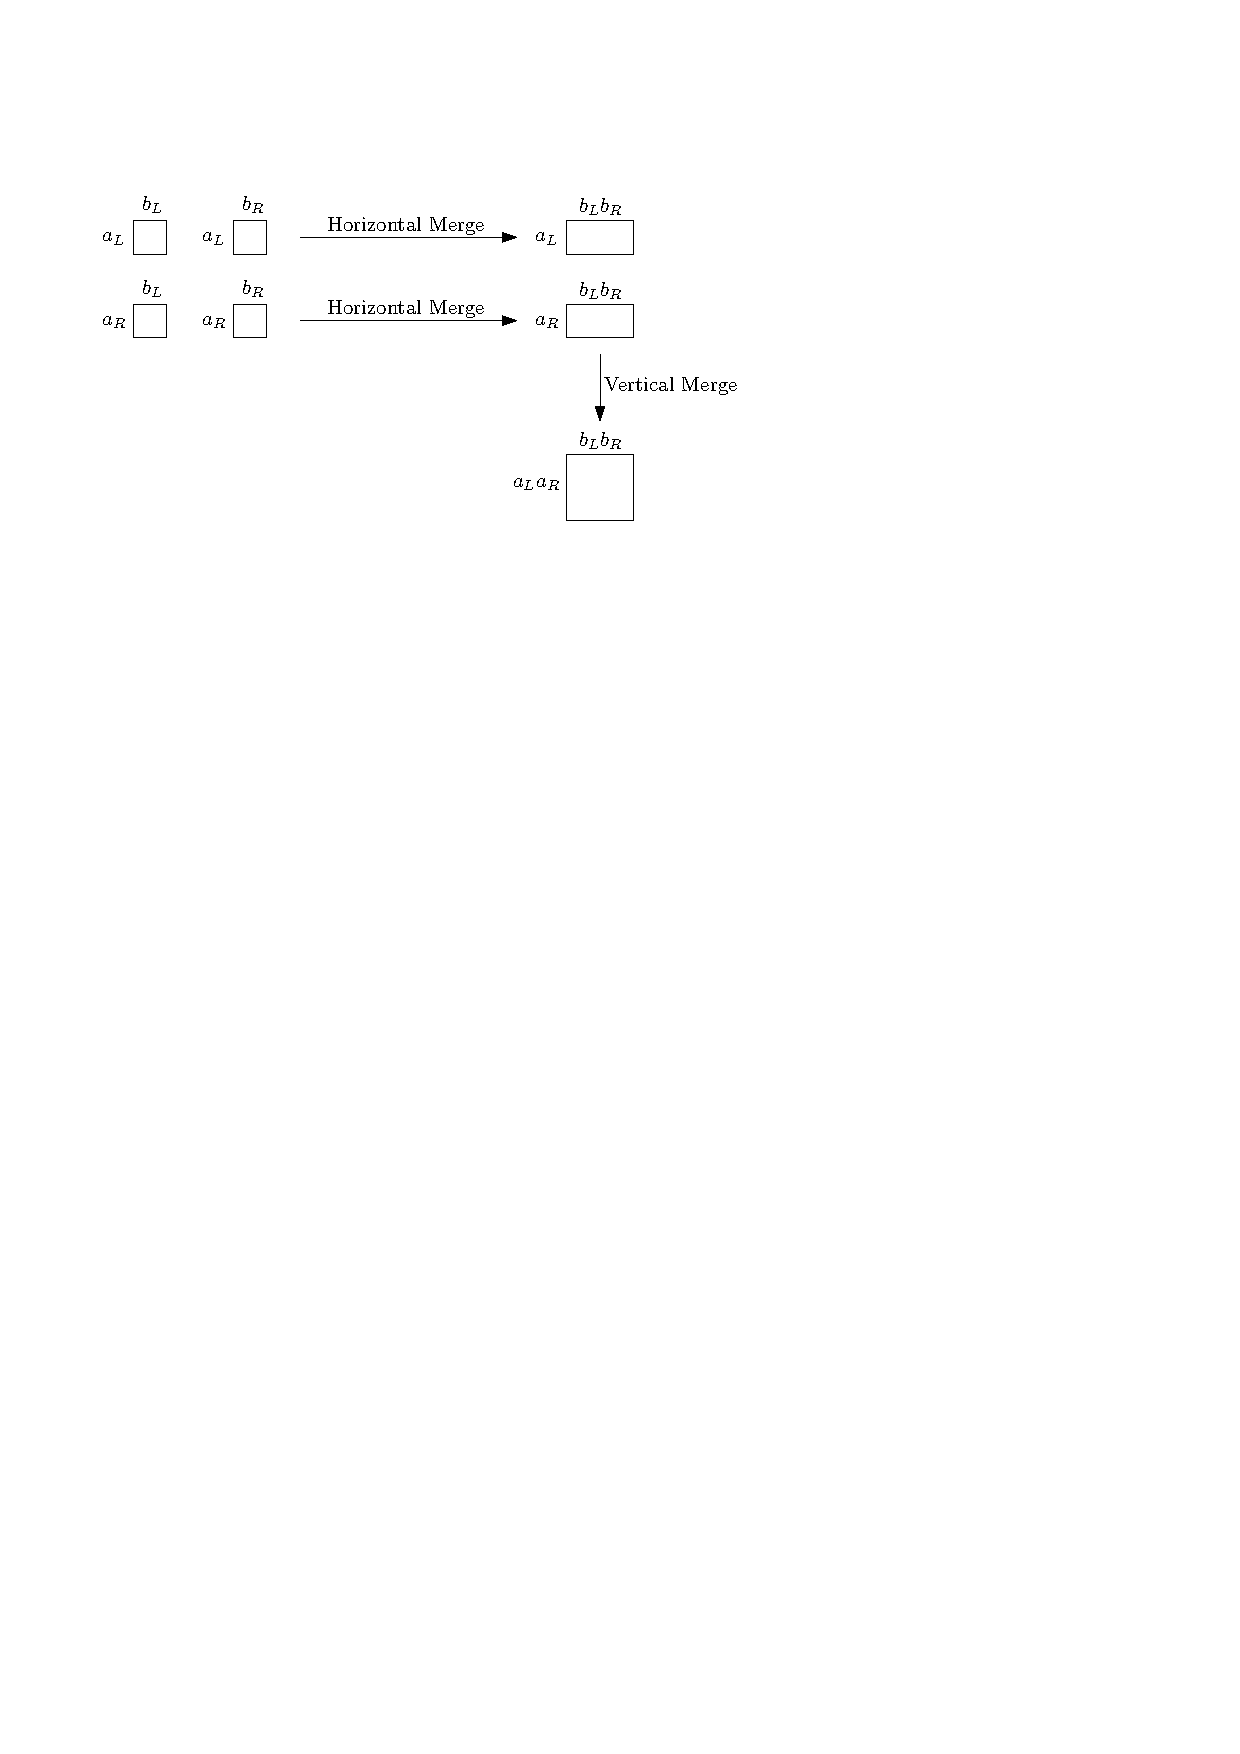
\includegraphics{images/dist_merge}
    \caption{Merging phases of DIST tables from the children to obtain the DIST for the concatenated strings.}
    \label{fig:compression:dist:merge}
  \end{figure}

  \item[Productions associated with substring] For this type of productions a merging approach is also employed. Depending on what side of the path the node was selected, its left/right child is chosen accordantly, and then they are recursively solved and merged together as in the previous case.
\end{description}
Since the number of productions is bounded by $O(n^2)$, the time for constructing the dist repository can be build in time $O(n^2 M(x))$ using memorization, where $M(x)$ denotes the time for merging two DIST tables, which for a rational scoring function and the succinct DIST representation takes time $O(x \log{x})$. In total $O(n^2x\log{x})$ time is spend.

\subsection{Filling out the dynamical programming table}
\label{sec:algorithm:filling-grid-overview}
The dynamical programming table is filled from top to bottom, left to right. This is done by keeping two columns of the table in memory (could be reduced to a little more than one column), and then $O(x)$ of a row. This specifies the inputs $I$ to the dist table, and the output can then be computed by
\begin{equation}
  \label{eqn:dist-application}
  O[j] = \min_i \{ I[i] + \DIST[i, j] \},
\end{equation}
since the DIST table stores the shortest path from input $i$ to output $j$. Evaluating the above formula directly for every input takes $O(x^2)$ time, which is too much.

If an explicit representation of the DIST tables is used, then this can be evaluated in time $O(x)$ using the SMAWK algorithm (however, this would increase the time needed for constructing the DIST tables).

\section{Representation of $\DIST$s}
As mentioned in the previous section, representing the $\DIST$s in a succinct way is crucial in order to obtain the desired running time \todo{some more trash talk?}.

Given two strings $A$ and $B$, a succinct representation of the LCS DIST tables should be constructed. By definition of the $\DIST$ tables \todo{ref} it is known that
\[
  \DIST_{A,B}[i, j] = \left\{
    \begin{array}{ll}
      lcs(\substr{A}{m - i}{m}, \substr{B}{0}{j})             & \text{if } i < m, j < n \\
      lcs(A, \substr{B}{i - m}{j})                            & \text{if } i \geq m, j < n \\
      lcs(\substr{A}{m - i}{m - (j - n)}, B)                  & \text{if } i < m, j \geq n \\
      lcs(\substr{A}{0}{m - (j - n)}, \substr{B}{i - m}{n})   & \text{if } i \geq m, j \geq n
    \end{array}
  \right. ,
\]
that is, the $\DIST$ can be summarized as the LCS between all prefix-suffix pairs of the two strings $A$ and $B$.
\todo{Should this be here? Consider other approaches. Discuss with Chr!} Notice that a $\DIST$ table is not well-defined for $i > j + m$ and $j > i + n$ since it corresponds to non-existing paths in the dynamic programming table. In all following calculations or statements these invalid index combinations should simply be considered as statements without any information.

A different way of describing the LCS between these prefix-suffix pairs, is by the following definition.

\begin{mydef}[\refbook{p.-48}{Definition 4.8}]
  \label{def:H-table}
  Let $\str{A}{0}{m}$ and $\str{B}{0}{n}$ be strings, then for $i, j \in \{ 0, \dots, m + n \}$
  \[
    H_{A,B}(i, j) := \begin{cases}
                        j - (i - m)                         & \text{if j < i - m} \\
                        lcs(A, \substr{?^mB?^m}{i}{j + m})  & \text{o/w}
                      \end{cases}
  \]
  where $? \not\in \Sigma$ denotes a wildcard character matching all other symbols.
\end{mydef}
The first case in the $H_{A,B}$ definition is introduced because of the entries in the corresponding $\DIST$ table that are not well-defined. The $H$-table entries corresponding to these undefined $\DIST$ entries is simply chosen to make everything work out as they should in able to make the $H$-tables easy representable. In almost all the following calculations is has been chosen not to include this case as it is straight forward that the choice will work.

The precise correspondence between the $H$-table of \cref{def:H-table} and the $\DIST$ tables, is given by the following lemma.
\begin{lemma}[\refbook{p.-48}{mentioned but not proved}]
  \label{lemma:dist-H-relation}
  \[
  DIST[i, j] = H(i, j) + \left\{
    \begin{array}{ll}
      i - m             & \text{if } i < m, j < n \\
      0                 & \text{if } i \geq m, j < n \\
      (i - m) + (n - j) & \text{if } i < m, j \geq n \\
      n - j             & \text{if } i \geq m, j \geq n
    \end{array}
  \right.
  \]
  \begin{proof}
    The lemma follows almost directly by the definition of the DIST, $H$-table and $lcs$ function, by splitting the claim up into the four different cases of the statement.
    \begin{description}
      \item[\circled{1}] For $i \in \{0, \dots, m\}, j \in \{0, \dots, n\}$,
       \begin{align*}
         H(i, j) &= lcs(A, \substr{?^mB?^m}{i}{j + m}) = lcs(A, ?^{m - i}(\substr{B}{0}{j})) \\
                 &= (m - i) + lcs(\substr{A}{m - i}{m}, \substr{B}{0}{j}) = \DIST[i, j] + m - i
       \end{align*}

      \item[\circled{2}] For $i \in \{m, \dots, m + n\}, j \in \{0, \dots, n\}$,
        \[
          H(i, j) = lcs(A, \substr{?^mB?^m}{i}{j + m}) = lcs(A, \substr{B}{i - m}{j}) = \DIST[i, j]
        \]

      \item[\circled{3}] For $i \in \{0, \dots, m\}, j \in \{n, \dots, n + m\}$,
        \begin{align*}
          H(i, j) &= lcs(A, \substr{?^mB?^m}{i}{j + m}) = lcs(A, ?^{m - i}B?^{j - n}) \\
                  &= (m - i) + (j - n) + lcs(\substr{A}{m - i}{m - (j - n)}, B) \\
                  & = (m - i) + (j - n) + \DIST[i, j]
        \end{align*}

      \item[\circled{4}] For $i \in \{m, \dots, m + n\}, j \in \{n, \dots, n + m\}$,
        \begin{align*}
          H(i, j) &= lcs(A, \substr{?^mB?^m}{i}{j + m}) = lcs(A, \substr{B}{i - m}{n}?^{j - n}) \\
                  &= (j - n) + lcs(\substr{A}{0}{m - (j - n)}, \substr{B}{i - m}{n}) = (j - n) + \DIST[i, j]
        \end{align*}
    \end{description}
  \end{proof}
\end{lemma}
An important property of the $H$-table is that it is almost simple unit-Monge.
\begin{lemma}[\refbook{p.-49}{Theorem 4.10}]
  \label{lemma:H-permutation-representation}
  Given a $H$-table $H$ satisfying \cref{def:H-table}, there exists a permutation matrix $P$ of size $m + n - 1$ such that
  \[
    H(i, j) = j - (i - m) - P^{\Sigma}(i, j).
  \]
  Therefore, the permutation matrix $P$, which can be represented in linear space, encodes the $H$-table, and thereby also the $\DIST$-table.

  \begin{proof}
    Define the following matrix to be a small pertubation of the $H$-table
    \[
      N(i, j) := j - (i - m) - H(i, j).
    \]
    We will prove that $N$ is simple unit-Monge by which the statement follows. First it will be shown that $N$ is Monge, that is $N^{\Box} \geq 0$. From the definition of $N$ and $\Box$ it is needed to show that
    \begin{align*}
      &H(i, j + 1) - H(i, j) - H(i + 1, j + 1) + H(i + 1, j) = H^{\Box}(i, j) \leq 0 \\
      \iff &H(i, j + 1) + H(i + 1, j) \leq H(i, j) + H(i + 1, j + 1)
    \end{align*}
    for all $i,j$. By \cref{def:H-table} the adjacent entries of the $H$-table in the above equation correspond to the LCS of a fixed string with a string where a character is possibly extended in both ends. The situation is illustrated in \cref{fig:H-permutation-representation:monge} where the top of the illustration corresponds to the left hand side of the inequality and the bottom corresponds to the right hand side.

    It is clear that the part between $i + 1$ and $j$ will always ensure some fixed contribution to all of the intervals. Now assume that the top contribution is strictly more than two times this fixed contribution. This can happen if it is possible to match an unmatched symbol by introducing cell $i$ or $j + 1$. It is easy to see that if this is the case, then it is easy to do the same for one (or both) of the bottom intervals. Therefore the bottom intervals will always match more than the top intervals, which gives the inequality and thereby the Monge property.
    \begin{figure}[h!]
      \centering
      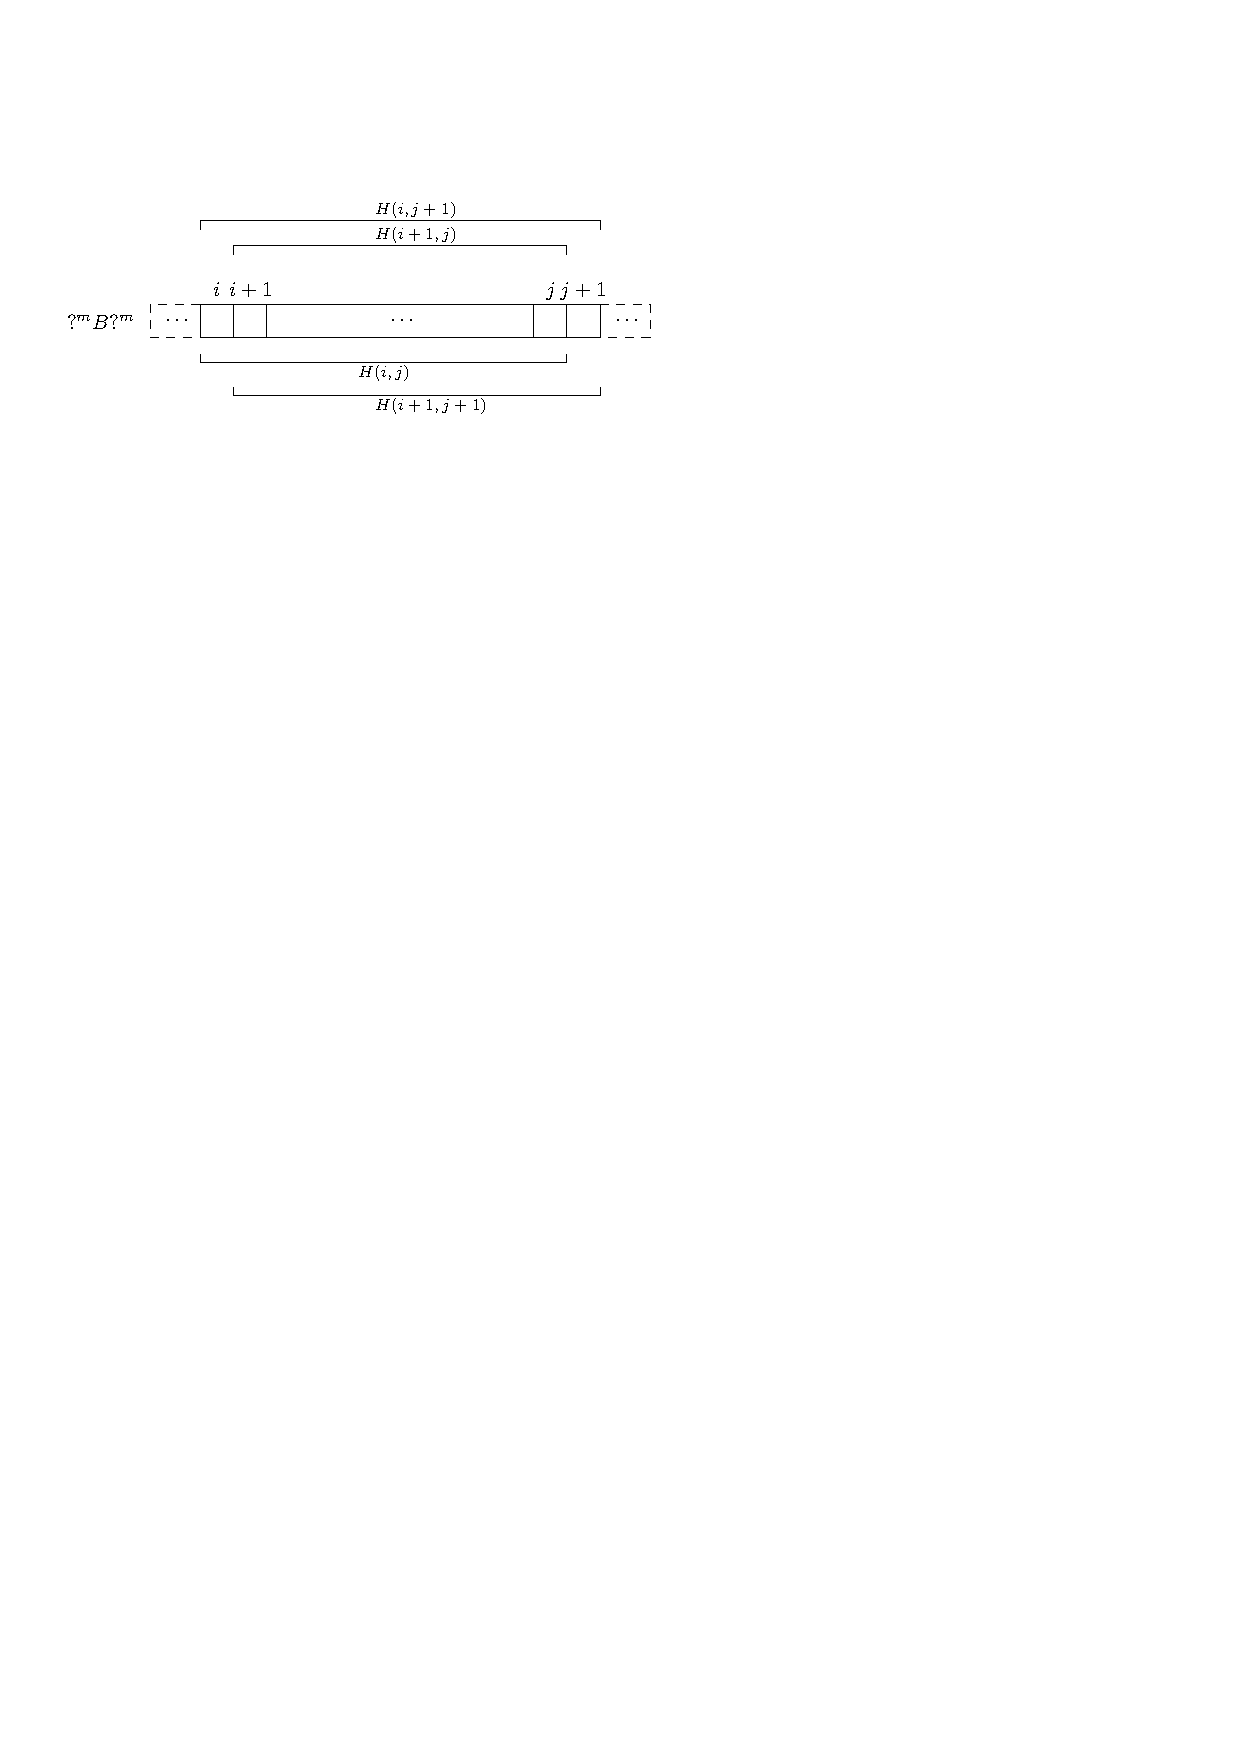
\includegraphics[width=11cm]{images/monge-condition-illustration}
      \caption{Illustration of how the longest common subsequence extension relates to the Monge property.}
      \label{fig:H-permutation-representation:monge}
    \end{figure}

    Note the following properties about $N$:
    \begin{align*}
      N(i, 0) &= 0 - (i - m) - H(i, j)
        = (m - i) - \begin{cases}
          0 - (i - m)                    & \text{if } i > m \\
          lcs(A, \substr{?^mB?^m}{i}{m}) & \text{o/w}
        \end{cases} \\
        &= (m - i) - (m - i) = 0
    \end{align*}
    \begin{align*}
      N(m + n, j) &= j - ((m + n) - m) - H(i, j) \\
        &= j - n - \begin{cases}
          j - n                                   & \text{if } j < n \\
          lcs(A, \substr{?^mB?^m}{m + n}{j + m})  & \text{o/w}
        \end{cases} \\
        &= (j - n) - (j - n) = 0
    \end{align*}
    Therefore \cref{claim:simple-matrix-characterization} gives that $N$ is a simple matrix. Also note that the following equalities hold for $i,j \in \{0, \dots, m + n\}$:
    \begin{align*}
      N&(i, n + m) - N(i + 1, n + m) \\
        &= (n + m - (i - m) - H(i, n + m)) - (n + m - ((i + 1) - m)) - H(i + 1, n + m) \\
        &= 1 - H(i, n + m) + H(i + 1, n + m) \\
        &= 1 - lcs(A, \substr{?^mB?^m}{i}{2m+n}) + lcs(A, \substr{?^mB?^m}{i + 1}{2m+n}) \\
        &= 1 - m + m = 1
    \\ \\
      N&(0, j + 1) - N(0, j) \\
        &= (j + 1 - (0 - m) - H(i, j + 1)) - (j - (0 - m) - H(i, j)) \\
        &= 1 - H(0, j + 1) + H(0, j) \\
        &= 1 - lcs(A, \substr{?^mB?^m}{0}{j + 1 + m}) + lcs(A, \substr{?^mB?^m}{0}{j + m}) \\
        &= 1 - m + m = 1
    \end{align*}
    Since $N$ is simple Monge and have the above properties \cref{lemma:unit-monge-characterization} gives that $N$ is unit-Monge.
  \end{proof}
\end{lemma}
What remains is to ensure that the merge and apply operations operations on the $\DIST$ table can be computed efficiently using only the permutation matrix representation.

\subsection{Merging of $\DIST$ tables}
The following definition will come in handy:
\begin{mydef}
  Let $P_{A'}$ and $P_{A''}$ be permutation matrices describing the $\DIST$ tables for the strings $\str{A'}{0}{m'}$ and $\str{A''}{0}{m''}$ respectively. Then define the following index change matrices
  \[
    IC'_{P_{A'}} = \begin{pmatrix}
      I^{m'' \times m''} & 0 \\
      0 & P_{A'}
    \end{pmatrix}, \quad
    IC''_{P_{A''}} = \begin{pmatrix}
      P_{A''} & 0 \\
      0 & I^{m' \times m'}
    \end{pmatrix}.
  \]
  Notice that both of these new matrices are also permutation matrices, and that they can be efficiently computed by a single scan of the original matrices.
\end{mydef}

The following convenient fact that will be useful later, follows directly from the definition of the $\Sigma$-operator:
\[
  {IC'_{P_{A'}}}^{\varsigma} = \begin{pmatrix}
    (I^{m'' \times m''})^{\varsigma} & \cdot \\
    0 & P_{A'}^{\varsigma}
  \end{pmatrix}, \quad
  {IC''_{P_{A''}}}^{\varsigma} = \begin{pmatrix}
    P_{A''}^{\varsigma} & \cdot \\
    0 & (I^{m' \times m'})^{\varsigma}
  \end{pmatrix},
\]
where $\varsigma$ denotes the $\Sigma$ operator, but where the last row and the first column are removed.

\subsubsection{Vertical merge}
Now it will be explained how a vertical merge between $A'$ and $A''$ can be found only giving the succinct representation of the DIST tables $\DIST_{A',B}$ and $\DIST_{A'',B}$. From a straight forward analysis of the LCS graph described by the $\DIST$ tables, it is found that:
\begin{claim}
  \label{claim:dist-vertical-merge}
  \item[\circled{1}]: For $i \leq m'', j \leq n + m''$:
    \[
      \DIST_{A'A'',B}[i, j] = \DIST_{A'',B}[i, j]
    \]
  \item[\circled{2}]: For $i \geq m'', j \geq n + m''$:
    \[
      \DIST_{A'A'',B}[i, j] = \DIST_{A',B}[i - m'', j - m''].
    \]
  \item[\circled{3}]: For $i \geq m'', j \leq n + m'$:
    \[
      \DIST[i, j] = \max_{k \in \{0, \dots, n\} } \left\{ \DIST_{A',B}[i - m'', k] + \DIST_{A'',B}[m'' + k, j] \right\}
    \]
  \begin{proof}
    Straight forward from the meaning of the $\DIST$ tables in term of the dynamic programming table by the simple LCS algorithm. \todo{Insert illustrative figure?}
  \end{proof}
\end{claim}
%
For case \circled{3}, the result from \cref{claim:dist-vertical-merge} can be further expanded to find
\begin{align*}
  \DIST_{A'A'',B}[i, j] &= \max_{k \in \{0, \dots, n\} } \left\{ \DIST_{A',B}[i - m'', k] + \DIST_{A'',B}[m'' + k, j] \right\} \\
              &=  \begin{aligned}
                    \max_k \left\{
                      H_{A',B}(i - m'', k) + \left\{
                        \begin{array}{ll}
                          i - m & \text{if } i - m'' < m' \\
                          0     & \text{o/w}
                        \end{array} \right. \right. \\
                      \left. +\,\,H_{A'',B}(m'' + k, j) + \left\{
                        \begin{array}{ll}
                          n - j & \text{if } j \geq n \\
                          0     & \text{o/w}
                        \end{array} \right.
                    \right\}
                 \end{aligned}\\
              &= \max_k \left\{ H_{A',B}(i - m'', k) + H_{A'',B}(m'' + k, j) \right\}
                  + \begin{cases}
                      (i - m) + (n - j)   & \text{if } i < m, j \geq n \\
                      i - m               & \text{if } i < m, j < n \\
                      n - j               & \text{if } i \geq m, j \geq n \\
                      0                   & \text{if } i \geq m, j < n
                    \end{cases}.
\end{align*}
Therefore \cref{lemma:dist-H-relation} now implies that $H_{A'A'',B}(i, j) = \max_k \left\{ H_{A',B}(i - m'', k) + H_{A'',B}(m'' + k, j) \right\}$. This expression can further be written out, to find
\begin{align*}
  H_{A'A'',B}(i, j) &= \max_k \left\{ H_{A',B}(i - m'', k) + H_{A'',B}(m'' + k, j) \right\} \\
                    &= \max_k \left\{ k - (i - m'' - m') - P_{A'}^{\Sigma}(i - m'', k) + j - (k + m'' - m'') - P_{A''}^{\Sigma}(k + m'', j) \right\} \\
                    &= j - (i - m) + \max_k \left\{ -\left( P_{A'}^{\Sigma}(i - m'', k) + P_{A''}^{\Sigma}(k + m'', j) \right)  \right\} \\
                    &= j - (i - m) - \min_k \left\{ P_{A'}^{\Sigma}(i - m'', k) + P_{A''}^{\Sigma}(k + m'', j) \right\}.
\end{align*}
Now \cref{lemma:H-permutation-representation} gives that
\begin{align*}
  P_{A'A''}^{\Sigma}(i, j) &= \min_k \left\{ P_{A'}^{\Sigma}(i - m'', k) + P_{A''}^{\Sigma}(k + m'', j) \right\} \\
                           &= \min_k \{ {IC'_{P_{A'}}}^{\Sigma}(i, k) + {IC''_{P_{A''}}}^{\Sigma}(k, j) \},
\end{align*}
which reduces this case to min-multiplying two simple unit-Monge matrices, which can be solved in time $O(n \log{n})$ by an algorithm given by \cite{Tiskin:2010:FDM:1873601.1873704} and described in \cref{sec:algorithm:min-mult-two-unit-monge}.

For case \circled{1} where $i \leq m'', j \leq n + m''$, the definition of the $\DIST$ table yields
\begin{align*}
  \DIST_{A'A'',B}[i, j] &= H_{A'A'',B}(i, j) + \left\{
    \begin{array}{ll}
      i - m             & \text{if } j < n \\
      (i - m) + (n - j) & \text{if } j \geq n
    \end{array}
  \right. \\
  &= (i - m) + j - (i - m) - P_{A'A'',B}^\Sigma(i, j) + \left\{
    \begin{array}{ll}
      0             & \text{if } j < n \\
      (n - j)       & \text{if } j \geq n
    \end{array}
  \right. \\
  &= j - P_{A'A'',B}(i, j) + \left\{
    \begin{array}{ll}
      0             & \text{if } j < n \\
      n - j         & \text{if } j \geq n
    \end{array}
  \right.
\end{align*}
By a similar analysis of the statement given by \cref{claim:dist-vertical-merge}, it is found that:
\begin{align*}
  \DIST_{A'A'',B}[i, j] &= \DIST_{A'',B}[i, j] = H_{A'',B}(i, j) + \left\{
    \begin{array}{ll}
      i - m''             & \text{if } j < n \\
      (i - m'') + (n - j) & \text{if } j \geq n
    \end{array}
  \right. \\
  &= \dots = j - P_{A'',B}^{\Sigma}(i, j) + \left\{
    \begin{array}{ll}
      0             & \text{if } j \geq n \\
      n - j         & \text{if } j < n
    \end{array}
  \right.
\end{align*}
Subtracting the two expressions yields $P_{A'',B}^{\Sigma}(i, j) = P_{A'A'',B}^{\Sigma}(i, j)$. It can be noticed that this conforms nicely with the computation carried out in case \circled{1}. Writing from the computation from case \circled{1},
\begin{align*}
  \circled{*} &= \min_{k \in \{0,\dots,n+m\}} \{ {IC'_{P_{A'}}}^{\Sigma}(i, k) + {IC''_{P_{A''}}}^{\Sigma}(k, j) \} \\
  &= \min\left\{
       \min_{k \in \{0,\dots,i\}}{P_{A'',B}^{\Sigma}(k, j)},
       \min_{k \in \{i + 1, n + m\}}\left\{ k - i + \left\{ % A row <= m'' in IC' is like: 0 ... 0 1 2 3 4 ...
        \begin{array}{ll}
          P_{A'',B}^{\Sigma}(k, j) & \text{if } k \leq n + m'' \\
          0                        & \text{if } k > n + m''
        \end{array}
       \right. \right\}
     \right\}.
\end{align*}
%
\begin{claim}
  \label{claim:bounding-sigma}
  The following bound is valid $\forall k \in \mathbb{N}: i + k \leq n + m''$:
  \[
    P_{A''}^{\Sigma}(i, j) \leq k + P_{A''}^{\Sigma}(i + k, j)
  \]
  \begin{proof}
    Follows almost directly from decreasing unit monotonicity of the $\Sigma$-operator used on permutation matrices in both coordinates (only the $i$ coordinate monotonicity used here).
  \end{proof}
\end{claim}
Using \cref{claim:bounding-sigma} at the boundary condition $i + k = n + m''$, it is found that $P_{A''}^{\Sigma}(i, j) \leq n + m'' - i + P_{A''}^{\Sigma}(n + m'', j) = n + m'' - i$. Hence, by first using decreasing unit monotonicity of the $\Sigma$-operator and \cref{claim:bounding-sigma} followed by the claim at the boundary condition, it is found that:
\[
  \circled{*} = \min\{ P_{A''}^{\Sigma}(i, j), \min_{k \in \{n+m'', \dots, n+m\}} \{ k - i \} \}
              = P_{A''}^{\Sigma}(i, j)
\]
Hence, the min-product computed in case \circled{3} also gives the correct result for case \circled{1}.

Case \circled{2} follows by almost the same arguments as case \circled{1}. First \cref{lemma:dist-H-relation} and the definition of the $H$-table is used on \cref{claim:dist-vertical-merge} yielding
\begin{align*}
  \DIST_{A'A'',B}[i, j] &= \DIST_{A',B}[i - m'', j - m''] \\
    &= H_{A',B}(i - m'', j - m'') +
      \begin{cases}
        (i - m'' - m') + (n - (j - m'')) & \text{if } i - m'' < m' \\
        n - (j - m'')                    & \text{if } i - m'' \geq m'
      \end{cases} \\
    &= n + m'' - j + H_{A',B}(i - m'', j - m'') +
      \begin{cases}
        i - m   & \text{if } i < m \\
        0       & \text{o/w}
      \end{cases} \\
    &= n - (i - m) - P_{A',B}^{\Sigma}(i - m'', j - m'') +
      \begin{cases}
        i - m   & \text{if } i < m \\
        0       & \text{o/w}
      \end{cases}
\end{align*}
Similarly writing out directly from the definition, it is found that
\begin{align*}
  \DIST_{A'A'',B}[i, j] &= H_{A'A'',B}(i, j) +
    \begin{cases}
      (i - m) + (n - j) & \text{if } i < m \\
      n - j             & \text{if } i \geq m
    \end{cases} \\
  &= n - (i - m) - P_{A'A'',B}^{\Sigma}(i, j) +
    \begin{cases}
      i - m & \text{if } i < m \\
      0     & \text{if } i \geq m
    \end{cases}
\end{align*}
This implies that $P_{A'A'',B}^{\Sigma}(i, j) = P_{A',B}^{\Sigma}(i - m'', j - m'')$. As will be seen, this is also what is computed by the min-multiplication in case \circled{3}. Writing out the result of the min-multiplication, it is found that
\begin{align*}
  \circled{*} &= \min_{k\in \{ 0, \dots, n + m \}} { {IC'_{P_{A'}}}^{\Sigma}(i, k) + {IC''_{P_{A''}}}^{\Sigma}(k, j) } \\
              &=  \begin{aligned} \min
                    &\left\{
                      \min_{k \in \{0, \dots, m''\}} { P_{A'}^{\Sigma}(k, n + m'') + I^{\Sigma}(0, j - (n + m'')) }, \right. \\
                    &\left.
                      \min_{k \in \{m', \dots, n + m''\}} {P_{A'}^{\Sigma}(i - m'', k - m'') + I^{\Sigma}(0, j - (n + m''))}, \right. \\
                    &\left.
                      \min_{k \in \{ n + m'', \dots, n + m \}} {P_{A'}^{\Sigma}(i - m'', k - m'') + I^{\Sigma}(k - (n + m''), j - (n + m''))}
                    \right\}
                  \end{aligned}
\end{align*}
Notice that the second case always dominates the first, hence the second case can safely be removed from the minimization. Furthermore, the third case can be spitted to obtain
\begin{align*}
  \circled{*} &=  \begin{aligned} \min
                    &\left\{
                      n + m'' + j - n - m'',
                      \min_{k \in \{n + m'', j\}} {j - k + P_{A'}^{\Sigma}(i - m'', k - m'')}, \right. \\
                    &\left.
                      \min_{k \in \{j, \dots, n + m\}} {P_{A'}^{\Sigma}(i - m'', k - m'')}
                    \right\}
                  \end{aligned} \\
              &= \begin{aligned} \min
                    &\left\{
                      j,\quad
                      \min_{k \in \{j, \dots, n + m\}} {j - k + P_{A'}^{\Sigma}(i - m'', k - m'')},\quad
                      P_{A'}^{\Sigma}(i - m'', j - m'')
                    \right\}
                  \end{aligned}
\end{align*}
\begin{claim}
  \label{claim:bounding-sigma-col}
  The following bound is valid $\forall a \in \mathbb{N}: j - a \geq 0$:
  \[
    P_{A'}^{\Sigma}(i - m'', j) \leq a + P_{A'}^{\Sigma}(i - m'', j - a)
  \]
  \begin{proof}
    Follows from unit monotonicity of the $\Sigma$-operator on permutation matrices.
  \end{proof}
\end{claim}
By applying \cref{claim:bounding-sigma-col} with $a = j - k$, it is found that
\[
  P_{A'}^{\Sigma}(i - m'', j - m'') \leq (j - k) + P_{A'}^{\Sigma}(i - m'', j - m'' - (j - k)) = (j - k) + P_{A'}^{\Sigma}(i - m'', k - m'').
\]
This eliminates the middle case of the minimization in $\circled{*}$. Moreover, \cref{claim:bounding-sigma-col} is used to find that
\[
  P_{A'}^{\Sigma}(i - m'', j - m'') \leq (j - m'') + P_{A'}^{\Sigma}(i - m'', 0) = j - m'' \leq j,
\]
which directly gives that $\circled{*} = P_{A'}^{\Sigma}(i - m'', j - m'')$. Therefore the min-multiplication can also be used to solve case \circled{2}. The above calculations establish the following important theorem.
\begin{theorem}[\refbook{p.-55}{Theorem 4.19}]
  Given two $\DIST$ tables $DIST_{A',B}$ and $\DIST_{A'',B}$ with representations $P_{A'}$ and $P_{A''}$ they can be merged into $\DIST_{A'A'',B}$ with representation $P_{A'A''}^{\Sigma}$ by setting
  \[
    P_{A'A''} = IC'_{P_{A'}} \boxdot IC''_{P_{A''}} .
  \]
\end{theorem}

 Therefore two $\DIST$ tables can be merged vertically by a single min-multiplication taking $O(x \log{x})$ time using the described in \cref{sec:algorithm:min-mult-two-unit-monge}.

\subsubsection{Horizontal merge}
The horizontal merge will be carried out by means of a vertical merge. In order to do this, it should be efficient to compute $\DIST_{B,A}$ from $\DIST_{A,B}$. It turns out that this indeed easy. In order to see this, first notice that
\begin{claim}[\refbook{p.-52}{Lemma 4.14, no proof}]
  \label{claim:H_string_switch_relation}
  For all $i, j \in \{0, \dots, n + m\}$ the following identity holds
  \[
    H_{A,B}(i, j) = (m - i) - (n - j) + H_{B,A}(n + m - i, n + m - j)
  \]
  \begin{proof}
    The proof is a case analysis of \cref{def:H-table}.
    \begin{description}
      \item[\circled{1}]: For $i \in \{0, \dots, m\}, j \in \{0, \dots, n\}$
        \begin{align*}
          H_{A,B}(i, j) &= (m - i) + lcs(\substr{A}{m - i}{m}, \substr{B}{0}{j}) \\
            &= (m - i) + lcs(\substr{B}{0}{j}, \substr{A}{m - i}{m}) \\
            &= (m - i) - (n - j) + lcs(B, \substr{A}{m - i}{m} ?^{n - j}) \\
            &= (m - i) - (n - j) + lcs(B, \substr{?^nA?^n}{n + m - i}{m + n + n - j}) \\
            &= (m - i) - (n - j) + H_{B,A}(n + m - i, n + m - j)
        \end{align*}

      \item[\circled{2}]: For $i \in \{m, \dots, m+n\}, j \in \{0, \dots, n\}$
        \begin{align*}
          H_{A,B}(i, j) &= lcs(A, \substr{B}{i - m}{j}) = lcs(\substr{B}{i - m}{j}, A) \\
            &= lcs(B, \substr{?^n A ?^n}{n - (i - m)}{n + m + (n - j)}) - (i - m) - (n - j) \\
            &= (m - i) - (n - j) + H_{B,A}(m + n - i, m + n - j)
        \end{align*}

      \item[\circled{3}]: For $i \in \{0, \dots, m\}, j \in \{n, \dots, n+m\}$
        \begin{align*}
          H_{A,B}(i, j) &= (m - i) - (n - j) + lcs(\substr{A}{m - i}{m - (j - n)}, B) \\
            &= (m - i) - (n - j) + lcs(B, \substr{?^n A ?^n}{m + n - i}{m + n - (j - n)}) \\
            &= (m - i) - (n - j) + H_{B,A}(m + n - i, m + n - j)
        \end{align*}

      \item[\circled{4}]: For $i \in \{m, \dots, m+n\}, j \in \{n, \dots, n+m\}$
        \begin{align*}
          H_{A,B}(i, j) &= (j - n+ lcs(\substr{A}{0}{m - (j - n)}, \substr{B}{i - m}{n})) \\
            &= (j - n) + lcs(\substr{B}{i - m}{n}, \substr{A}{0}{m + n - j}) \\
            &= (j - n) + lcs(B, \substr{?^n A ?^n}{n - (i - m)}{n + m + n - j}) - (i - m) \\
            &= (m - i) - (n - j) + H_{B,A}(n + m - i, m + n - j)
        \end{align*}
    \end{description}
  \end{proof}
\end{claim}
%
\begin{claim}
  \label{claim:sum_top_described_as_sum_bottom}
  For all $i, j \in \{0, \dots, n + m\}$ it is the case that
  \[
    \sum_{\substack{ \hat{i} \in \{i, \dots, n + m - 1\} \\ \hat{j} \in \{ 0, \dots, j - 1 \}}} P_{B,A}(m + n - \hat{i}, m + n - \hat{j})
      = j - i + P_{B,A}^{\Sigma}(m + n - i, m + n - j)
  \]
  \begin{proof}
    Since $P_{B,A}$ is a permutation matrix, it contains exactly one $1$ in every row/column. Therefore the sum over the top-right area, can be found by taking the sum over the entire matrix and subtract the left and bottom part, and then add the double counted overlap \todo{See figure ...}. This gives that
    \begin{align*}
      &\sum_{\substack{ \hat{i} \in \{i, \dots, n + m - 1\} \\ \hat{j} \in \{ 0, \dots, j - 1 \}}} P_{B,A}(m + n - \hat{i}, m + n - \hat{j}) \\
      = &(n + m) - (m + n - j) - ((m + n) - (m + n - i)) + P_{B,A}^{\Sigma}(m + n - i, m + n - j) \\
      = &j - i + P_{B,A}^{\Sigma}(m + n - i, m + n - j).
    \end{align*}
  \end{proof}
\end{claim}

\begin{lemma}[\refbook{p.-52}{Lemma 4.14, no proof}]
  \label{lemma:swap_strings}
  Assuming $P_{A,B}$ is the permutation matrix encoding $\DIST_{A,B}$, the $\DIST$-table $\DIST_{B,A}$ is encoded by the permutation matrix $P_{B,A}$ where,
  \[
    P_{B,A}(m + n - i, m + n - j) = P_{A,B}(i, j).
  \]
  Notice that the transformed permutation matrix $P_{B,A}$ can easily be computed in linear time by a sweep over its rows.
  \begin{proof}
    It is needed to show that the $H$-table corresponding to the permutation matrix $P_{B,A}$ conforms to \cref{claim:H_string_switch_relation}.
    \begin{align*}
      H_{A,B}(i, j) &= j - (i - m) - P_{A,B}^{\Sigma}(i, j) \\
        &= j - (i - m) - \sum_{\substack{ \hat{i} \in \{i,\dots,n+m - 1\} \\ \hat{j} \in \{0, \dots, j - 1\}}} P_{A,B}(\hat{i}, \hat{j}) \\
        &= j - (i - m) - \sum_{\substack{ \hat{i} \in \{i, \dots, n + m - 1\} \\ \hat{j} \in \{ 0, \dots, j - 1 \}}} P_{B,A}(m + n - \hat{i}, m + n - \hat{j}) \\
        &\overset{\text{\cref{claim:sum_top_described_as_sum_bottom}}}{=} j - (i - m) - (j - i + P_{B,A}^{\Sigma}(m + n - i, m + n - j)) \\
        &= m - P_{B,A}^{\Sigma}(m + n - i, m + n - j) \\
        &= m - \left( (n + m - j) - ((n + m - i) - n) - H_{B,A}(n + m - i, n + m - j) \right) \\
        &= (m - i) - (n - j) + H_{B,A}(n + m - i, n + m - j)
    \end{align*}
    This matches the statement of \cref{claim:H_string_switch_relation}, which completes the proof.
  \end{proof}
\end{lemma}
%
Following \cref{lemma:swap_strings} a horizontal merge can be carried out by first swapping the strings, then performing a vertical merge, and then swapping the strings of the merged $\DIST$ table again. Since swapping the strings runs in time $O(x)$, the total time of a horizontal merge is bounded by the time of the vertical merging. Hence, the total time of either of the merge routines is bounded by $O(x\log{x})$.

\subsection{Application of $\DIST$ tables}
When filling out a block in the grid with input $I$, the output is given by
\begin{align*}
  O[j] &= \max_i \left\{ I[i] + \DIST[i, j] \right\} \\
    &= \max_i \left\{ I[i] + H(i, j) + \left\{
      \begin{array}{ll}
        i - m             & \text{if } i < m, j < n \\
        0                 & \text{if } i \geq m, j < n \\
        (i - m) + (n - j) & \text{if } i < m, j \geq n \\
        n - j             & \text{if } i \geq m, j \geq n
      \end{array}
    \right. \right\} \\
    &= \max_i\left\{ \left( I[i] + \left\{
      \begin{array}{ll}
        i - m     & \text{if } i < m \\
        0         & \text{o/w.}
      \end{array}
    \right. \right) + H(i, j) \right\} + \left\{
      \begin{array}{ll}
        n - j     & \text{if } j \geq n \\
        0         & \text{o/w.}
      \end{array}
    \right. .
\end{align*}
Hence, the output can be evaluated by max-multiplying the $H$ table with a slight perturbation of the input array, followed by an addition for every resulting output. \cite{Gawrychowski:2012:FAC:2422024.2422048} gave a linear time algorithm for max-multiplying an arbitrary vector with a $H$-table which is described in \cref{sec:algorithm:max-mult-H-table-with-vector}. This gives a linear time algorithm for applying a $\DIST$ table.

\section{Efficient simple unit-Monge operations}

\subsection{Min-multiplication of two simple unit-Monge matrices}
\label{sec:algorithm:min-mult-two-unit-monge}
\todo{Description / proof of the algorithm.}

\subsection{Max-multiplication of $H$-table with vector}
\label{sec:algorithm:max-mult-H-table-with-vector}
\todo{Description / proof of the algorithm.}

\subsubsection{Interval Union Find}
\label{sec:algorithm:interval-union-find}
\todo{Describe the algorithm.}

As mentioned in the description of the algorithm, an interval union find data-structure is required. The data-structure implemented is the one of \cite{Itai06lineartime}, where every operation takes amortized constant time. Note however that the amortized constant time relies on blocking the input into blocks of size $\Theta(\log{n})$. In the actual implementation, it has been chosen to always use block sizes of machine word $64$ bits, which in practice is a constant. This choice will always perform superior in practice due to practical limit on the input size, but the theoretical running time of the algorithm becomes \todo{calculate this}.

\section{Benchmarks}

From the benchmark section of the string compression chapter (\cref{sec:compression:benchmarks}), it was found that almost all "real-world" strings, was only compressible by a constant factor (up to the trivial repetition of the string due to the fixed alphabet size \todo{experiment / comment on this?} \todo{Argue that this effect is negligible in practice (empirically determined on DNA input), and that the $\sqrt{\log{\frac{N}{n}}}$ parts eats most of the advantage}). That is, for all realistic DNA related applications it has empirically been found that $n = cN$ for some $c \in \mathbb{R}$. In this case, the running times of the algorithm is
\[
  O\left( nN\sqrt{\log{\frac{N}{n}}} \right) = O\left( c \cdot N^2 \sqrt{\log{\frac{N}{cN}}} \right) = O(N^2),
\]
which is also the running time of the simple algorithm. Therefore the practical success of the implemented algorithm becomes a battle of constants against the simple algorithm, which it is very likely going to lose. One approach to overcome this problem may be to improve the way the strings are compress, and try to make different inputs share the same SLP, a little more elaboration on this idea is done in the section on further work in \cref{chapter:conclusion}.


\chapter{Conclusion}
\label{chapter:conclusion}
Summarize findings.

\section{Further work}
\label{sec:conclusion:further-work}
During the project, a number of ideas for potentially improving (mostly of practical concerns) the approach of computing edit distance based on SLPs have been considered. These ideas are shortly described and motivated in the following list:

\begin{itemize}
  \item Parallelization of the algorithm: The two SLP representations can easily be computed in parallel. Inside the construction of the SLPs the parallelization is not obvious.
  For the expensive parts of the algorithm (constructing the DISTs and filling the dynamical programming grid), parallelization is easy. For construction of the dist, parallelization can be applied to every invocation of \texttt{build}, which happens for every pair of selected SLP productions and every recursive call.
  For filling out the grid, the algorithm can be parallelized in the same way as the simple algorithm, by choosing a suitable order to fill out the blocks.

  \item The algorithm for min-multiplying two unit-Monge matrices runs in time $O(n \log{n})$, however no lower bound other than $\Omega(n)$ is known. It could be interesting to close this gap. If is is possible to make a $\Theta(n)$ algorithm, the time for building the DIST tables can be reduced to $O(n^2 x)$, and by picking $x = \frac{N}{n}$, the total running time of the algorithm becomes $O(\underbrace{n^2 x}_{\DIST} + \underbrace{\frac{N^2}{x}}_{\text{Grid}}) = O(nN)$, which is an asymptotic improvement.

  \item Consider if the compressed strings could be reused, such that a lot of compressed strings can be entangled into one SLP. This would make it possible for a lot of strings to share DIST tables, and also possible do a better compression of highly similar strings. This could be of interest when computing the edit distance between all pairs of a large number of sequences, which is useful when approximating a phylogeny from sequence data.

  \item As mentioned in \cref{ch:compressing-strings}, the space consumption of the SLP has a very high constant when measured in terms of the number of productions in the SLP. As mentioned in the report, this is directly will not make the approach applicable to strings not compressing well, however a succinct representation of the SLP for given strings may be of interest in other problems working on SLPs.
\end{itemize}

%%%%%%%%%%%%%%%%%%%%%%%%%%%%%%%%%%%%%%%%%%%%%%%%%%%%%%%%%%%%%%%%%%%%%%%

\addcontentsline{toc}{chapter}{Bibliography}
\bibliographystyle{plain} 
\bibliography{refs}
%\addcontentsline{toc}{chapter}{Secondary Bibliography}
%\bibliographystyleB{plain} 
%\bibliographyB{refs} % remove this if you don't need secondary literature

\end{document}

